%%%%%%%%%%%%%%
%% Run LaTeX on this file several times to get Table of Contents,
%% cross-references, and citations.

%% If you have font problems, you may edit the w-bookps.sty file
%% to customize the font names to match those on your system.

%% w-bksamp.tex. Current Version: Feb 16, 2012
%%%%%%%%%%%%%%%%%%%%%%%%%%%%%%%%%%%%%%%%%%%%%%%%%%%%%%%%%%%%%%%%
%
%  Sample file for
%  Wiley Book Style, Design No.: SD 001B, 7x10
%  Wiley Book Style, Design No.: SD 004B, 6x9
%
%
%  Prepared by Amy Hendrickson, TeXnology Inc.
%  http://www.texnology.com
%%%%%%%%%%%%%%%%%%%%%%%%%%%%%%%%%%%%%%%%%%%%%%%%%%%%%%%%%%%%%%%%

%%%%%%%%%%%%%
% 7x10
%\documentclass{wileySev}

% 6x9
\documentclass{wileySix}

\usepackage{graphicx}
\usepackage{listings}
\usepackage{float}

\usepackage{color}

\definecolor{codegreen}{rgb}{0,0.6,0}
\definecolor{codegray}{rgb}{0.5,0.5,0.5}
\definecolor{codepurple}{rgb}{0.58,0,0.82}
\definecolor{backcolour}{rgb}{0.95,0.95,0.92}

\lstdefinestyle{mystyle}{
    backgroundcolor=\color{backcolour},
    commentstyle=\color{codegreen},
    keywordstyle=\color{magenta},
    numberstyle=\tiny\color{codegray},
    stringstyle=\color{codepurple},
    basicstyle=\footnotesize,
    breakatwhitespace=false,
    breaklines=true,
    captionpos=b,
    keepspaces=true,
    numbers=left,
    numbersep=5pt,
    showspaces=false,
    showstringspaces=false,
    showtabs=false,
    tabsize=2,
    language=sh
}

\lstset{style=mystyle}

%%%%%%%
%% for times math: However, this package disables bold math (!)
%% \mathbf{x} will still work, but you will not have bold math
%% in section heads or chapter titles. If you don't use math
%% in those environments, mathptmx might be a good choice.

% \usepackage{mathptmx}

% For PostScript text
\usepackage{w-bookps}

%%%%%%%%%%%%%%%%%%%%%%%%%%%%%%%%%%%%%%%%%%%%%%%%%%%%%%%%%%%%%%%%
%% Other packages you might want to use:

% for chapter bibliography made with BibTeX
% \usepackage{chapterbib}

% for multiple indices
% \usepackage{multind}

% for answers to problems
% \usepackage{answers}

%%%%%%%%%%%%%%%%%%%%%%%%%%%%%%
%% Change options here if you want:
%%
%% How many levels of section head would you like numbered?
%% 0= no section numbers, 1= section, 2= subsection, 3= subsubsection
%%==>>
\setcounter{secnumdepth}{3}

%% How many levels of section head would you like to appear in the
%% Table of Contents?
%% 0= chapter titles, 1= section titles, 2= subsection titles,
%% 3= subsubsection titles.
%%==>>
\setcounter{tocdepth}{2}

%% Cropmarks? good for final page makeup
%% \docropmarks

%%%%%%%%%%%%%%%%%%%%%%%%%%%%%%
%
% DRAFT
%
% Uncomment to get double spacing between lines, current date and time
% printed at bottom of page.
% \draft
% (If you want to keep tables from becoming double spaced also uncomment
% this):
% \renewcommand{\arraystretch}{0.6}
%%%%%%%%%%%%%%%%%%%%%%%%%%%%%%

%%%%%%% Demo of section head containing sample macro:
%% To get a macro to expand correctly in a section head, with upper and
%% lower case math, put the definition and set the box
%% before \begin{document}, so that when it appears in the
%% table of contents it will also work:

\newcommand{\VT}[1]{\ensuremath{{V_{T#1}}}}

%% use a box to expand the macro before we put it into the section head:

\newbox\sectsavebox
\setbox\sectsavebox=\hbox{\boldmath\VT{xyz}}

%%%%%%%%%%%%%%%%% End Demo


\begin{document}


\booktitle{Cerdas Menguasai Python}
\subtitle{Dalam 24 Jam}

\authors{Rolly M. Awangga\\
\affil{Informatics Research Center}
%Floyd J. Fowler, Jr.\\
%\affil{University of New Mexico}
}

\offprintinfo{Cerdas Menguasai Python, First Edition}{Rolly M. Awangga}

%% Can use \\ if title, and edition are too wide, ie,
%% \offprintinfo{Survey Methodology,\\ Second Edition}{Robert M. Groves}

%%%%%%%%%%%%%%%%%%%%%%%%%%%%%%
%%
\halftitlepage

%\titlepage


\begin{copyrightpage}{2019}
\input{info/copyrightpage}
\end{copyrightpage}

\dedication{`Jika Kamu tidak dapat menahan lelahnya belajar,
Maka kamu harus sanggup menahan perihnya Kebodohan.'
~Imam Syafi'i~}

\begin{contributors}
\input{info/contributors}
\end{contributors}

\contentsinbrief
\tableofcontents
\listoffigures
\listoftables
\lstlistoflistings


\begin{foreword}
\input{info/foreword}
\end{foreword}

\begin{preface}
\input{info/preface}
\end{preface}


\begin{acknowledgments}
\input{info/acknowledgments}
\end{acknowledgments}

\begin{acronyms}
\input{info/acronyms}
\end{acronyms}

\begin{glossary}
\input{info/glossary}
\end{glossary}

\begin{symbols}
\input{info/symbols}
\end{symbols}

\begin{introduction}
\input{info/introduction}
\end{introduction}

%%%%%%%%%%%%%%%%%%Isi Buku_
%TEORI
%\chapter{Judul Bagian Pertama}
%\input{chapters/Teori/1}
%PRAKTEK
%\chapter{Judul Bagian Pertama}
%\input{chapters/Praktek/1}

%TEORI
%\chapter{Judul Bagian Pertama}
%\input{chapters/Teori/2}
%PRAKTEK
%\chapter{Judul Bagian Pertama}
%\input{chapters/Praktek/2}

%TEORI
%\chapter{Judul Bagian Pertama}
%\input{chapters/Teori/3}
%PRAKTEK
%\chapter{Judul Bagian Pertama}
%\input{chapters/Praktek/3}

%TEORI
%\chapter{Library CSV dan Pandas}
%
\section{Muhammad Afra Faris/1174041}
\subsection{Soal 1}
Fungsi, Sejarah, dan Contoh file CSV : 
\begin{itemize}
	\item Fungsi : 
	File Comma Separated Values atau  biasa disingkat dengan CSV merupakan tipe file khusus yang menyimpan informasi dengan metode dipisahkan dengan koma. File CSV berfungsi untuk menjadi perantara beberapa aplikasi yang memiliki basis data saat pengiriman data. CSV juga dapat dibuka di berbagai text editor. Dengan bentuk filenya yang dinamis, file CSV mungkin dapat dimanipulasi dan dapat menyimpan informasi dengan skala besar.
	\item Sejarah :
	CSV ini sudah digunakan sejak tahun 1972 yang dapat dikompilasi pada bahasa pemrograman IBM Fortran. Pada saat itu, data yang dipisahkan oleh koma jika isinya memiliki spasi maka harus diberi tanda petik di awal dan akhir isi dari data tersebut. Nama CSV ini baru mulai digunakan pada tahun 1983. Pada panduan dari Osborne Executive Computer mendokumentasikan kutipan yang membolehkan isi karakter memiliki koma.  Tahun 2005 dengan RFC4180, CSV didefinisikan sebagai MIME Content Type. lalu pada tahun 2013, defisiensi dari RFC4180 dipecahkan oleh rekomendasi dari W3C. Tahun 2014, IETF mempublikasi RFC7111 yang mendeskripsikan pecahan Uniform Resource Identifier(URI) ke dokumen CSV. RFC7111 menjelaskan bagaimana baris, kolom dapat dipilih dalam dokumen CSV menggunakan indeks posisi. Pada Tahun 2015,  draft rekomendasi untuk CSV-metadata standards dipublikasikan W3C yang dimulai dengan rekomendasi pada bulan Desember dengan tahun yang sama. 
	\item Contoh File CSV \begin{itemize}
							\item 
							CSV pada Excel \ref{csvex}
							\begin{figure}[!htbp]
								\centering
								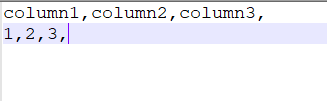
\includegraphics[height=4cm, width=7cm]{figures/4/1174041/Teori/csvex.png}
								\caption{Contoh CSV Pada Excel}
								\label{csvex}
							\end{figure}
														
						  \end{itemize}
\end{itemize}
\subsection{Soal 2}
Aplikasi Yang dapat membuat file CSV : 
Berikut file yang dapat membuat file CSV
\begin{itemize}
	\item Spreadsheet :
	Spreadsheet adalah aplikasi yang bisa digunakan membuat CSV hanya dengan memasukan data sesuai baris dan kolom yang diinginkan. Contoh dari spreadsheet seperti Microsoft Excel, Google Spreadsheet, dan beberapa aplikasi lainnya. 
	\item Bahasa Pemrograman :
	Bahasa pemrograman adalah sarana media yang dapat digunakan untuk membuat aplikasi, yang bisa membuat file CSV khusus untuk bahasa pemrograman yang mendukung dengan pembuatan file CSV. Seperti Python, C Sharp, dan lain sebagainya.
	\item Text Editor :
	Text editor juga dapat digunakan untuk membuat file CSV. Untuk membuat file CSV dengan Text Editor cukup dengan membuat file sesuai format CSV dan save file tersebut dengan ekstensi .CSV.
\end{itemize}
\subsection{Soal 3}
Menulis dan Membaca file CSV : 
Berikut cara menulis dan membaca file CSV : 
\begin{itemize}
	\item Menulis : \begin{enumerate}
						\item Buka file CSV dengan spreadsheet apapun
						\item Klik Cell yang akan dimasukkan
						\item Masukan data yang akan dimasukkan pada cell tersebut
						\item Lalu save file dengan format .CSV
					\end{enumerate}
	\item Membaca : \begin{enumerate}
						\item Buka file CSV dengan spreadsheet						
					\end{enumerate}
\end{itemize}
\subsection{Soal 4}
Sejarah Library CSV Python : 
Library CSV pada python merupakan library yang paling umum untuk import export data pada spreadsheet dan basis data dengan format sesuai dengan standarisasi RFC4180. Seiring dengan lahirnya bahasa pemrograman python, library mulai dibuat dan dikembangkan sampai akhirnya pada tahun 2003, pembuatnya Kevin Altis dan lainnya telah merilis versi final untuk library Python CSV. 
\subsection{Soal 5}
Sejarah Library Pandas Python : 
Pandas (Python Data Analysis Library) adalah library open source yang digunakan untuk melakukan data manajemen dan data analysis. Pandas diciptakan pada tahun 2008 oleh Wes McKinney dan diperbaharui oleh Sien Chang pada tahun 2010. Inspirasi dari pembuatan pandas muncul pada komunitas yang membutuhkan library khusus untuk analisis data. 
\subsection{Soal 6}
Fungsi - fungsi yang terdapat di library CSV : 
\begin{itemize}
	\item \begin{verbatim} csv.reader(csvfile, dialect='excel', **fmtparams) \end{verbatim} Untuk mengembalikan	object reader yang akan mengambil setiap line pada csv yang diambil. Data setiap baris diambil saat next() dipanggil. 
	\item \begin{verbatim} csv.writer(csvfile, dialect='excel', **fmtparams) \end{verbatim} Mengembalikan file pembuat object untuk dapat mengkonversi data pada python ke file CSV yang akan dibuat. 
	\item \begin{verbatim} csv.register_dialect(name[, dialect[, **fmtparams]]) \end{verbatim} Mengasosiasikan dialek dengan nama, dan nama yang dimasukkan harus berupa karakter.
	\item \begin{verbatim} csv.unregister_dialect(name) \end{verbatim}
	Menghapus asosiasi dialek dengan nama yang ada pada registry dialek.
	\item \begin{verbatim} csv.get_dialect(name) \end{verbatim}
	Mengambil dialek yang telah diasosiasikan dengan nama. 
	\item \begin{verbatim}  csv.list_dialects() \end{verbatim} Mengembalikan dialek yang telah terregistrasi.
	\item \begin{verbatim} csv.field_size_limit([new_limit]) \end{verbatim} Mengembalikan maksimal column data yang diperbolehkan oleh pembaca.
\end{itemize}
\subsection{Soal 7}
Fungsi - fungsi yang terdapat di library Pandas : 
\begin{itemize}
	\item \begin{verbatim} pandas.read_excel(io[, sheet_name, header, names, …])  \end{verbatim} Membaca file excel dan menyimpan ke DataFrame.
	\item \begin{verbatim} pandas.read_csv(filepath_or_buffer[, sep, …]) \end{verbatim} Untuk membaca file CSV dan menyimpan ke DataFrame.
	\item \begin{verbatim} to_csv([path, index, sep, na_rep, …]) \end{verbatim}
	Untuk membuat file CSV dari data yang telah ada.	
\end{itemize}
\subsection{Cek Plagiarism}
Berikut pengecekan plagiarism yang dilakukan pada website smallseotools.com : 
\begin{figure}[!htbp]
	\centering
	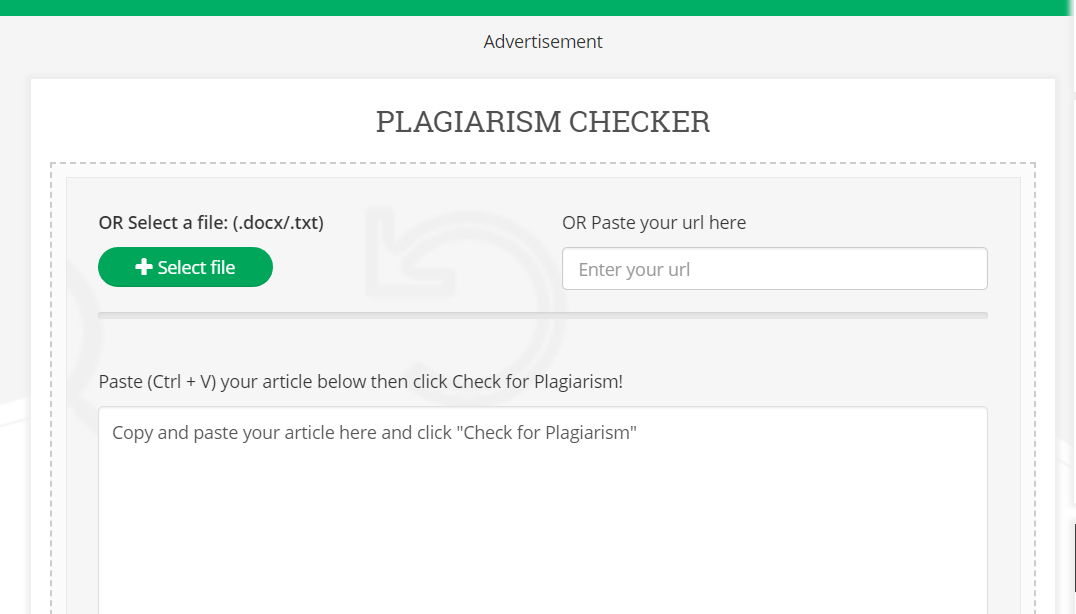
\includegraphics[height=6cm, width=10cm]{figures/4/1174041/Teori/plagiarism.png}
	\caption{Cek Plagiarisme}
	\label{plagiarism}
\end{figure}

\section{Rangga Putra Ramdani}
\subsection{Fungsi Csv}
Fungsi csv yaitu memudahkan user dalam melakukan input data karena pada csv input data ataupun import data dalam skala besar dapat dilakukan dengan cara yang sederhana.
\subsection{Sejarah Csv}
Dari rilis pertama, Excel menggunakan format file biner yang disebut Binary Interchange File Format (BIFF) sebagai format file utamanya. Ini berubah ketika Microsoft merilis Office System 2007 yang memperkenalkan Office Open XML sebagai format file utamanya. Office Open XML adalah file kontainer berbasis XML yang mirip dengan XML Spreadsheets (XMLSS), yang diperkenalkan di Excel 2002. File versi XML tidak bisa menyimpan makro VBA. Meskipun mendukung format XML baru, Excel 2007 masih mendukung format lama yang masih berbasis BIFF tradisional. Selain itu Microsoft Excel juga mendukung format Comma Separated Values (CSV), DBase File (DBF), SYMbolic LinK (SYLK), Format Interchange Data (DIF) dan banyak format lainnya, termasuk format lembar kerja 1-2 Lotus - 3 (WKS, WK1, WK2, dll.) Dan Quattro Pro.
\lstinputlisting[firstline=7, lastline=20]{src/4/1174056/teori/Shasa.py}
\subsection{Aplikasi yang dapat menghasilkan csv}
\begin{itemize}
\item Texteditor
Seperti notepad++,visual studio code,atom,sublime dan lain sebagainya
\item Program Spreadsheet
  Seperti excell,google spreadshare,LibreOfficecalc
 \end{itemize}
\subsection{Jelaskan bagaimana cara menulis dan membaca file csv di excel atau spreadsheet}
Caranya sangat mudah yaitu:
 Untuk menulisnya untuk yang paling atas itu kita buat headernya,untuk mepermudah membedakan datanya,dan untuk baris kedua dan seterusnya itu untuk data itu sendiri.Setelah di buat kalian save as kemudian pilih format CSV.Untuk membukan cukup di double clik file tersebut
\subsection{Jelaskan sejarah library csv}
CSV muncul untuk memudahkan data science dan analis karena dinilai terdapat banyak kemudahan yang didapat. CSV dapat dimaksimalkan jika dipaduka dengan python karena python adalah bahasa pemrograman yang support ke banyak library termasuk csv. Maka karena itulah perpaduan python dan csv seringkali digunakan oleh perusahaan-perushaan besar dalam mengolah datanya.
\subsection{Jelaskan sejarah library pandas}
Pandas merupakan tool yang dapat digunakan sebagai alat analisis data dan struktur untuk bahasa pemrograman Python. Pandas dapat mengolah data dengan mudah, salah satu fitur yang ada dalam pandas adalah Dataframe. Fitur dataframe dapat membaca sebuah file dan menjadikannya tabble, juga dapat mengolah suatu data dengan menggunakan operasi seperti join, group by dan teknik lainnya yang terdapat pada SQL. Dalam hal ini pandas tidak jauh beda dengan csv yaitu memiliki keunggulan dalam pengolahan data-data besar dan dapat disupport dengan baik dengan python walaupun mengimport data dalam jumlah banyak.
\subsection{Fungsi-fungsi Library CSV}
Dalam library csv terdapat dua fungsi yaiut fungsi membaca file dan menulis file csv.
Library csv mempunyai keunggulan dibandingkan format data lainnya adalah soal kompatibilitas. File csv dapat digunakan, diolah, diekspor/impor, dan dimodifikasi menggunakan berbagai macam perangkat lunak dan bahasa pemrograman. Pada library csv mempunyai fungsi import dan eksport data yang baik dan bisa digunakan dalam jumlah besar.
\subsection{Fungsi-fungsi library Pandas}
Pandas pun memiliki fungsi yang sama yaitu menulis dan membaca file. pandas menyediakan beragam fungsi operasi untuk mengolah data. Contoh jika menggunakan series bisa mencari nilai max, min, dan mean secara langsung, bahkan juga bisa melakukan operasi perpangkatan pada nilai Series secara langsung.
Pandas dapat mengolah suatu data dan mengolahnya seperti join, distinct, group by, agregasi, dan teknik seperti pada SQL. Hanya saja dilakukan pada tabel yang dimuat dari file ke RAM.

\section{Teddy Gideon Manik}
\subsection{Soal 1}
Comma Separated Value atau CSV adalah format data yang memudahkan penggunanya melakukan input data ke database secara sederhana. CSV dapat digunakan dalam standar file ASCII. Dalam format csv record dipisahkan dengan tanda koma atau titik koma. Ketika user menerima file dengan format CSV, yang biasanya bertuliskan .CSV, maka file tersebut akan terbuka dalam format Microsoft Excel. CSV muncul demi memenuhi kebutuhan perusahaan-perusahaan besar dalam mengolah data yang banyak.
\lstinputlisting[firstline=7, lastline=20]{src/4/1174038/teori/coba.py}
\subsubsection{Fungsi}
Fungsi csv yaitu memudahkan user dalam melakukan input data karena di csv input data atau import data dalam skala besar dapat dilakukan dengan cara yang sederhana.
\subsection{Soal 2}
Ada beberapa aplikasi yang dapat menghasilkan file dengan format csv diantaranya google sheet, number di MacOS dan microsoft excel.
\subsection{Soal 3}
cara membuat file csv di excel cukup mudah yaitu :
\begin{itemize}
	\item Buat foldernya
	\item Pilih save as
	\item pilih file dengan format csv
\end{itemize}
cara membaca file di csv :
\begin{itemize}
	\item Klik data get external data form text
	\item Akan muncul Text Import Wizard, arahkan pada file csv yang ingin anda buka Open.
	\item Setelah File terbuka, akan muncul Text Import Wizard.
	\item Pilih Delimited, Kemudian Next (Di sini, bisa juga menentukan baris awal yang akan di import)
	\item Centrang pada Tab dan Comma (Atau sesuai pengaturan File Anda) Next.
	\item Atur Format data pada tiap kolom yang tampil dan klik Finish
\end{itemize}
\subsection{Soal 4}
CSV muncul untuk memudahkan data science dan analis karena dinilai terdapat banyak kemudahan yang didapat. CSV dapat dimaksimalkan jika dipaduka dengan python karena python adalah bahasa pemrograman yang support ke banyak library termasuk csv. Maka karena itulah perpaduan python dan csv seringkali digunakan oleh perusahaan-perushaan besar dalam mengolah datanya.
\subsection{Soal 5}
Pandas merupakan tool yang dapat digunakan sebagai alat analisis data dan struktur untuk bahasa pemrograman Python. Pandas dapat mengolah data dengan mudah, salah satu fitur yang ada dalam pandas adalah Dataframe. Fitur dataframe dapat membaca sebuah file dan menjadikannya tabble, juga dapat mengolah suatu data dengan menggunakan operasi seperti join, group by dan teknik lainnya yang terdapat pada SQL. Dalam hal ini pandas tidak jauh beda dengan csv yaitu memiliki keunggulan dalam pengolahan data-data besar dan dapat disupport dengan baik dengan python walaupun mengimport data dalam jumlah banyak.
\subsection{Soal 6}
Dalam library csv terdapat dua fungsi yaiut fungsi membaca file dan menulis file csv.
Library csv mempunyai keunggulan dibandingkan format data lainnya adalah soal kompatibilitas. File csv dapat digunakan, diolah, diekspor/impor, dan dimodifikasi menggunakan berbagai macam perangkat lunak dan bahasa pemrograman. Pada library csv mempunyai fungsi import dan eksport data yang baik dan bisa digunakan dalam jumlah besar.
\subsection{Soal 7}
Pandas pun memiliki fungsi yang sama yaitu menulis dan membaca file. pandas menyediakan beragam fungsi operasi untuk mengolah data. Contoh jika menggunakan series bisa mencari nilai max, min, dan mean secara langsung, bahkan juga bisa melakukan operasi perpangkatan pada nilai Series secara langsung.
Pandas dapat mengolah suatu data dan mengolahnya seperti join, distinct, group by, agregasi, dan teknik seperti pada SQL. Hanya saja dilakukan pada tabel yang dimuat dari file ke RAM.

\section{Harun Ar-Rasyid}
\subsection{Soal 1}
Isi jawaban soal ke-1

Kalau mau dibikin paragrap \textbf{cukup enter aja}, tidak usah pakai \verb|par| dsb

%\subsection{Soal 2}
%Isi jawaban soal ke-2

%\subsection{Soal 3}
%Isi jawaban soal ke-3

\section{Sri Rahayu}
\subsection{Soal 1}
Isi jawaban soal ke-1

Kalau mau dibikin paragrap \textbf{cukup enter aja}, tidak usah pakai \verb|par| dsb

%\subsection{Soal 2}
%Isi jawaban soal ke-2

%\subsection{Soal 3}
%Isi jawaban soal ke-3

\section{Doli Jonviter}
\subsection{Soal 1}
Isi jawaban soal ke-1

Kalau mau dibikin paragrap \textbf{cukup enter aja}, tidak usah pakai \verb|par| dsb

%\subsection{Soal 2}
%Isi jawaban soal ke-2

%\subsection{Soal 3}
%Isi jawaban soal ke-3

\section{Rahmatul Ridha}
\subsection{Soal 1}
Isi jawaban soal ke-1

Kalau mau dibikin paragrap \textbf{cukup enter aja}, tidak usah pakai \verb|par| dsb

%\subsection{Soal 2}
%Isi jawaban soal ke-2

%\subsection{Soal 3}
%Isi jawaban soal ke-3

\section{Tomy Prawoto}
\subsection{Soal 1}
Isi jawaban soal ke-1

Kalau mau dibikin paragrap \textbf{cukup enter aja}, tidak usah pakai \verb|par| dsb

%\subsection{Soal 2}
%Isi jawaban soal ke-2

%\subsection{Soal 3}
%Isi jawaban soal ke-3


%PRAKTEK
%\chapter{Praktek Library CSV dan Pandas}
%\section{Rangga Putra Ramdani}
\subsection{Soal 1}
Berikut adalah pemanggilan file csv dengan library csv yang menggunakan list
\lstinputlisting[firstline=10, lastline=20]{src/4/1174056/praktek/c_1174056_csv.py}

\subsection{Soal 2}
Berikut adalah pemanggilan file csv dengan library csv yang menggunakan dictionary
\lstinputlisting[firstline=22, lastline=31]{src/4/1174056/praktek/c_1174056_csv.py}

\subsection{Soal 3}
Berikut adalah pemanggilan file csv dengan library pandas yang menggunakan list
\lstinputlisting[firstline=9, lastline=11]{src/4/1174056/praktek/p_1174056_pandas.py}

\subsection{Soal 4}
Berikut adalah pemanggilan file csv dengan library pandas yang menggunakan dictionary
\lstinputlisting[firstline=13, lastline=16]{src/4/1174056/praktek/p_1174056_pandas.py}

\subsection{Soal 5}
Berikut penggunaan untuk merubah standar penulisan tanggal, yang mengikuti standar penulisan dari pandas.
\lstinputlisting[firstline=18, lastline=20]{src/4/1174056/praktek/p_1174056_pandas.py}

\subsection{Soal 6}
Berikut merupakan pergantian index kolom
\lstinputlisting[firstline=22, lastline=24]{src/4/1174056/praktek/p_1174056_pandas.py}

\subsection{Soal 7}
berikut merupakan penggunaan untuk merename atribut yang digunakan, atau merubah nama header 0
\lstinputlisting[firstline=26, lastline=30]{src/4/1174056/praktek/p_1174056_pandas.py}

\subsection{Soal 8}
\lstinputlisting[firstline=8, lastline=10]{src/4/1174056/praktek/main_shasa.py}

\subsection{Soal 9}
\lstinputlisting[firstline=11, lastline=14]{src/4/1174056/praktek/main_shasa.py}

\subsection{Penanganan Error}
Dalam praktek kali ini alhamdulliah tidak menemukan error


\section{Teddy Gideon Manik}
\subsection{Soal 1}
Berikut adalah pemanggilan file csv dengan library csv yang menggunakan list
\lstinputlisting[firstline=10, lastline=20]{src/4/1174038/praktek/c_1174038_csv.py}

\subsection{Soal 2}
Berikut adalah pemanggilan file csv dengan library csv yang menggunakan dictionary
\lstinputlisting[firstline=22, lastline=31]{src/4/1174038/praktek/c_1174038_csv.py}

\subsection{Soal 3}
Berikut adalah pemanggilan file csv dengan library pandas yang menggunakan list
\lstinputlisting[firstline=9, lastline=11]{src/4/1174038/praktek/p_1174038_pandas.py}

\subsection{Soal 4}
Berikut adalah pemanggilan file csv dengan library pandas yang menggunakan dictionary
\lstinputlisting[firstline=13, lastline=16]{src/4/1174038/praktek/p_1174038_pandas.py}

\subsection{Soal 5}
Berikut penggunaan untuk merubah standar penulisan tanggal, yang mengikuti standar penulisan dari pandas.
\lstinputlisting[firstline=18, lastline=20]{src/4/1174038/praktek/p_1174038_pandas.py}

\subsection{Soal 6}
Berikut merupakan pergantian index kolom
\lstinputlisting[firstline=22, lastline=24]{src/4/1174038/praktek/p_1174038_pandas.py}

\subsection{Soal 7}
berikut merupakan penggunaan untuk merename atribut yang digunakan, atau merubah nama header 0
\lstinputlisting[firstline=26, lastline=30]{src/4/1174038/praktek/p_1174038_pandas.py}

\subsection{Soal 8}
\lstinputlisting[firstline=8, lastline=10]{src/4/1174038/praktek/main_teddy.py}

\subsection{Soal 9}
\lstinputlisting[firstline=11, lastline=14]{src/4/1174038/praktek/main_teddy.py}

\subsection{Penanganan Error}
Dalam praktek kali ini alhamdulliah tidak menemukan error

\section{Harun Ar-Rasyid}
\subsection{Soal 1}
Isi jawaban soal ke-1

\section{Mhd Zulfikar Akram Nasution}
\subsection{Membaca file csv pada lib csv dengan mode list}
\lstinputlisting[firstline=1, lastline=9]{src/4/1164081/Praktek/1164081_csv.py}

\subsection{ Membaca file csv pada lib csv dengan mode dictionary}
\lstinputlisting[firstline=11, lastline=16]{src/4/1164081/Praktek/1164081_csv.py}

\subsection{Membaca file csv pada lib pandas dengan mode list}
\lstinputlisting[firstline=1, lastline=7]{src/4/1164081/Praktek/1164081_pandas.py}

\subsection{Membaca file csv pada lib pandas dengan mode dictionary}
\lstinputlisting[firstline=9, lastline=13]{src/4/1164081/Praktek/1164081_pandas.py}

\subsection{Mengubah format tanggal menjadi standar DataFrame}
\lstinputlisting[firstline=15, lastline=18	]{src/4/1164081/Praktek/1164081_pandas.py}
	
\subsection{Mengubah index kolom}
\lstinputlisting[firstline=21, lastline=25]{src/4/1164081/Praktek/1164081_pandas.py}

\subsection{Mengubah atribut atau nama kolom}
\lstinputlisting[firstline=26, lastline=30]{src/4/1164081/Praktek/1164081_pandas.py}

\subsection{Membuat program NPM\_main.py dan isikan bagaimana cara membaca file csv dan membuat file csv}
\lstinputlisting[firstline=1, lastline=6]{src/4/1164081/Praktek/1164081_main.py}
	
\subsection{Membuat program NPM\_main2.py dan isikan bagaimana cara membaca file csv dan membuat file csv dengan lib pandas}
\lstinputlisting[firstline=1, lastline=6]{src/4/1164081/Praktek/1164081_main2.py}
	
Kalau mau dibikin paragrap \textbf{cukup enter aja}, tidak usah pakai \verb|par| dsb

%\subsection{Soal 2}
%Isi jawaban soal ke-2

%\subsection{Soal 3}
%Isi jawaban soal ke-3

\section{Sri Rahayu}
\subsection{Soal 1}
Isi jawaban soal ke-1

Kalau mau dibikin paragrap \textbf{cukup enter aja}, tidak usah pakai \verb|par| dsb

%\subsection{Soal 2}
%Isi jawaban soal ke-2

%\subsection{Soal 3}
%Isi jawaban soal ke-3

\section{Doli Jonviter}
\subsection{Soal 1}
Isi jawaban soal ke-1

Kalau mau dibikin paragrap \textbf{cukup enter aja}, tidak usah pakai \verb|par| dsb

%\subsection{Soal 2}
%Isi jawaban soal ke-2

%\subsection{Soal 3}
%Isi jawaban soal ke-3

\section{Rahmatul Ridha}
\subsection{Soal 1}
Isi jawaban soal ke-1

Kalau mau dibikin paragrap \textbf{cukup enter aja}, tidak usah pakai \verb|par| dsb

%\subsection{Soal 2}
%Isi jawaban soal ke-2

%\subsection{Soal 3}
%Isi jawaban soal ke-3

\section{Tomy Prawoto}
\subsection{Soal 1}
Isi jawaban soal ke-1

Kalau mau dibikin paragrap \textbf{cukup enter aja}, tidak usah pakai \verb|par| dsb

%\subsection{Soal 2}
%Isi jawaban soal ke-2

%\subsection{Soal 3}
%Isi jawaban soal ke-3


%TEORI
\chapter{PySerial}
\section{Liyana Majdah Rahma}
{\Large \textbf{Pemahaman Teori}}
\subsection{Soal No. 1}
Apa itu fungsi device manager di windows dan folder /dev di linux?

\hfill \break
Device Manager  dapat  membantu dalam mengelola  semua hardware yang terpasang  dalam suatu sistem Windows. 
 Berikut fungsi kegunaan Device Manager antara lain adalah :
\begin{enumerate}
	\item Menunjukkan status suatu hardware.
	\item Menunjukkan informasi detil suatu hardware.
	\item Mengelola driver hardware
	\item Disable dan Enable hardware
	\item Mengidentifikasi konflik antar perangkat keras.
\end{enumerate}

\hfill \break
Folder /bin merupakan isi program binner yang harus ada apabila sistem yang dipasang dalam mode single-user, dan juga  ada beberapa program penting seperti bash.

\subsection{Soal No. 2}
Jelaskan langkah-langkah instalasi driver dari arduino!

\hfill \break
Berikut ini adalah langkah-langkah instalasi driver dari Arduino UNO di Windows:

\begin{enumerate}
	\item Langkah pertama Hubungkan sistem minimun Arduino Uno ke komputer dengan kabel USB .
	\item Lalu pada bagian kanan didesktop PC , akan muncul popup “Installing device driver software” seperti pada gambar dibawah ini.
	\item Kemudian jika sistem  operasi Windows tidak menyediakan driver untuk Arduino Uno,maka harus  melakukan instalasinya harus dilakukan secara manual.
	\item Lalu  Buka Device Manager,  dengan cara pada bagian Search Program and Files lalu ketikkan “device manager” (tanpa tanda petik). 
	\item kemudian Pada bagian COntrol Panel akan muncul Device Manager, lalu klik untuk menjalankan program tersebut.
	\item Setelah itu cari  Unknown device pada bagian Other device, biasanya terdapat tanda seru berwarna kuning, itu disebabkan karena penginstallan gagal.
	\item Klik kanan pada bagian  “Unknown device” kemudian pilih Update Driver Software.
	\item kemudian cari Browse my computer for driver software pada laptop anda.
	\item setelah itu lakukan dengan mengklik Install pada tampilan Windows Security.
	\item Jika instalasi driver pada laptop anda berhasil maka akan muncul Windows has successfully updated your driver software.
	\item Perhatikan dan ingat nama COM Arduino Uno, karena nama COM ini yang akan digunakan untuk meng-upload program nantinya
\end{enumerate}

\subsection{Soal No. 3}
Jelaskan bagaimana cara membaca baudrate dan port dari komputer yang sudah terinstall driver!

\hfill \break
\textbf{Membaca Port dari Komputer}

\begin{enumerate}
	\item Hubungkan modul TX-RX serial dengan komputer melalui serial port menggunakan DB9 cable extension.
	\item Buka Hyper Terminal dengan menekan start kemudian All progams lalu Accessories kemudian Communications lalu Hyper Terminal.
	\item Ketik nama untuk Connection Description, misal coba, kemudian tekan OK.
	\item Pada Connect to, pilihlah COM port yang dipakai di Connect using, kemudian tekan OK.
	\item Masukkan nilai-nilai port settingnya, sesuai dengan DCE-nya. Kemudian tekan OK.
\end{enumerate}



\subsection{Soal No. 4}
Jelaskan sejarah library pyserial!.

\hfill \break
PySerial adalah library/modul Python siap-pakai dan gratis yang dibuat untuk memudahkan kita dalam membuat program komunikasi data serial RS232 dalam bahasa Python.

\subsection{Soal No. 5}
Jelaskan fungsi-fungsi apa saja yang dipakai dari library pyserial!

\hfill \break
Fungsi-fungsi yang dipakai dari library PySerial, yaitu:
\begin{enumerate}
	\item Serial - fungsi ini untuk membuka port serial.
	\item write(data) - fungsi ini menulis data lewat port serial.
	\item readline() - fungsi ini membaca sebuah string dari port serial.
	\item read(size) - fungsi ini untuk membaca jumlah byte dari port serial.
	\item close() - fungsi ini untuk menutup port serial.
\end{enumerate}

\subsection{Soal No. 6}
Jelaskan kenapa butuh perulangan dan tidak butuh perulangan dalam membaca serial!

\hfill \break
Pada saat membaca serial di Arduino diperlukan perulangan agar dapat membaca data secara berulang kali sehingga data yang muncul banyak. Sedangkan apabila tidak membutuhkan perulangan maka Arduino hanya akan membaca data sekali saja.

\subsection{Soal No. 7}
Jelaskan bagaimana cara membuat fungsi yang mengunakan pyserial!

\hfill \break
Fungsi yang berada pada Python, dibuat dengan nama kata kunci def kemudian diikuti dengan nama fungsinya pada pyhton.
Seperti halnya dengan blok kode yang lain, kita juga harus memberikan identasi untuk menuliskan isi fungsi.

\section{Rangga Putra Ramdhani}
\subsection{ Apa itu fungsi device manager di windows dan folder /dev di linux}
Device Manager adalah Panel Kontrol dalam sistem operasi Microsoft Windows. Ini memungkinkan pengguna untuk melihat dan mengontrol perangkat keras yang terpasang pada komputer. Ketika beberapa bagian perangkat keras tidak berfungsi, perangkat keras yang terkait akan disorot oleh pengguna. Daftar perangkat keras dapat disortir berdasarkan berbagai kriteria.
Untuk setiap perangkat, pengguna dapat:
\begin{itemize}
     \item Menyediakan driver perangkat sesuai dengan Model Driver Windows
     \item Aktifkan atau nonaktifkan perangkat
     \item Beri tahu Windows untuk mengabaikan perangkat yang tidak berfungsi
     \item Lihat sifat teknis lainnya
\end{itemize}
Device Manager diperkenalkan dengan Windows 95 dan kemudian ditambahkan ke Windows 2000. Dalam versi berbasis NT, ini dimasukkan sebagai snap-in Konsol Manajemen Microsoft.\newline

/ dev adalah lokasi file khusus atau perangkat. Ini adalah direktori yang sangat menarik yang menyoroti satu aspek penting dari sistem file Linux - semuanya adalah file atau direktori.


\subsection{Jelaskan langkah-langkah instalasi driver dari Arduino}
Berikut ini merupakan langkah-langkah untuk melakukan instalasi driver Arduino
\begin{itemize}
	\item Pertama-tama, pasang board arduino pada pc. Kemudian tunggu sampai windows mencoba menginstal sendiri. jika gagal, lanjutkan ke step selanjutnya
	\item buka Device Manager 
	\item Cari nama arduino atau "Unknown Device"
	\item klik kanan pada unknown device , dan pilih update software
	\item Cari folder instalan software arduino
	\item klik Next
	\item Jika telah berhasil, maka proses instal driver sudah selesai
\end{itemize}

\subsection{Jelaskan bagaimana cara membaca baudrate dan port dari komputer yang sudah terinstal driver}
Berikut ini merupakan cara membaca baudrate dan port dari komputer yang sudah terinstal driver :
\begin{itemize}
	\item Sambungkan port USB arduino dengan port USB pc
	\item Kemudian buka software arduino pada pc
	\item Setelah itu, pilih tipe arduino yang digunakan
	\item Kemudian memilih serial port yang aktif  
	\item Selanjutnya untuk memasukkan program pada arduino, klik tombol upload
	\item Setelah proses upload selesai, buka fitur serial monitor
	\item Lalu sesuaikan Baudrate pada serial monitor dengan Baudrate yang terdapat pada program
\end{itemize}

\subsection{Jelaskan sejarah library pyserial}
Pyserial berguna untuk merangkum akses untuk port serial. Pyserial menyediakan backends untuk Python yang berjalan di Windows, Linux, BSD (mungkin sistem yang mendukung POSIX), Jython dan IronPython (.NET dan Mono). Modul bernama "serial" secara otomatis memilih backend yang sesuai. Antarmuka berbasis kelas yang sama pada semua platform yang didukung.
Akses ke pengaturan port melalui properti Python.
Dukungan untuk berbagai ukuran byte, bit stop, paritas dan kontrol aliran dengan RTS / CTS dan / atau Xon / Xoff.
Bekerja dengan atau tanpa menerima batas waktu.
File seperti API dengan "read" dan "write" ("readline" dll. Juga didukung).
File-file dalam paket ini adalah 100 persen Python murni.
Port diatur untuk transmisi biner. Tidak ada stripping byte NULL, terjemahan CR-LF dll. (Yang berkali-kali diaktifkan untuk POSIX.) Ini membuat modul ini bermanfaat secara universal.
Kompatibel dengan pustaka io (Python 2.6+)

\subsection{Jelaskan fungsi-fungsi apa saja yang dipakai dari library pyserial}
Serial – fungsi ini untuk membuka port serial
Write(data) – untuk menulis data lewat port serial
Readline() – untuk membaca string dari port serial
Read(size) – untuk membaca jumlah byte dari port serial
Close() – ini untuk menutup port serial 

\subsection{Jelaskan kenapa butuh perulangan dalam tidak butuh perulangan dalam membaca serial}
Perualangan dalam bahasa pemrograman berfungsi menyuruh komputer melakukan sesuatu secara berulang-ulang. Terdapat dua jenis perualangan dalam bahasa pemrograman python, yaitu perulangan dengan for dan while.
Perulangan for disebut counted loop (perulangan yang terhitung), sementara perulangan while disebut uncounted loop (perulangan yang tak terhitung). Perbedaan yang terlihat adalah pada perulangan for digunakan untuk mengulangi kode yang sudah diketahui banyak perulangannya. Sedangkan perulangan while digunakan pada perulangan yang memiliki syarat dan tidak tentu berapa banyak perulangannya.
Perulangan diperlukan agar dapat membaca data secara berulang kali sehingga data yang muncul lebih dari satu.  Sedangkan apabila tidak memakai perulangan maka data akan terbaca satu kali saja.

\subsection{Jelaskan bagaimana cara membuat fungsi yang mengunakan pyserial}
Fungsi yang berada pada Python, dibuat dengan nama kata kunci def kemudian diikuti dengan nama fungsinya pada pyhton.
Seperti halnya dengan blok kode yang lain, kita juga harus memberikan identasi untuk menuliskan isi fungsi.

\subsection{Plagiarisme}
\begin{figure}[h]
\centering
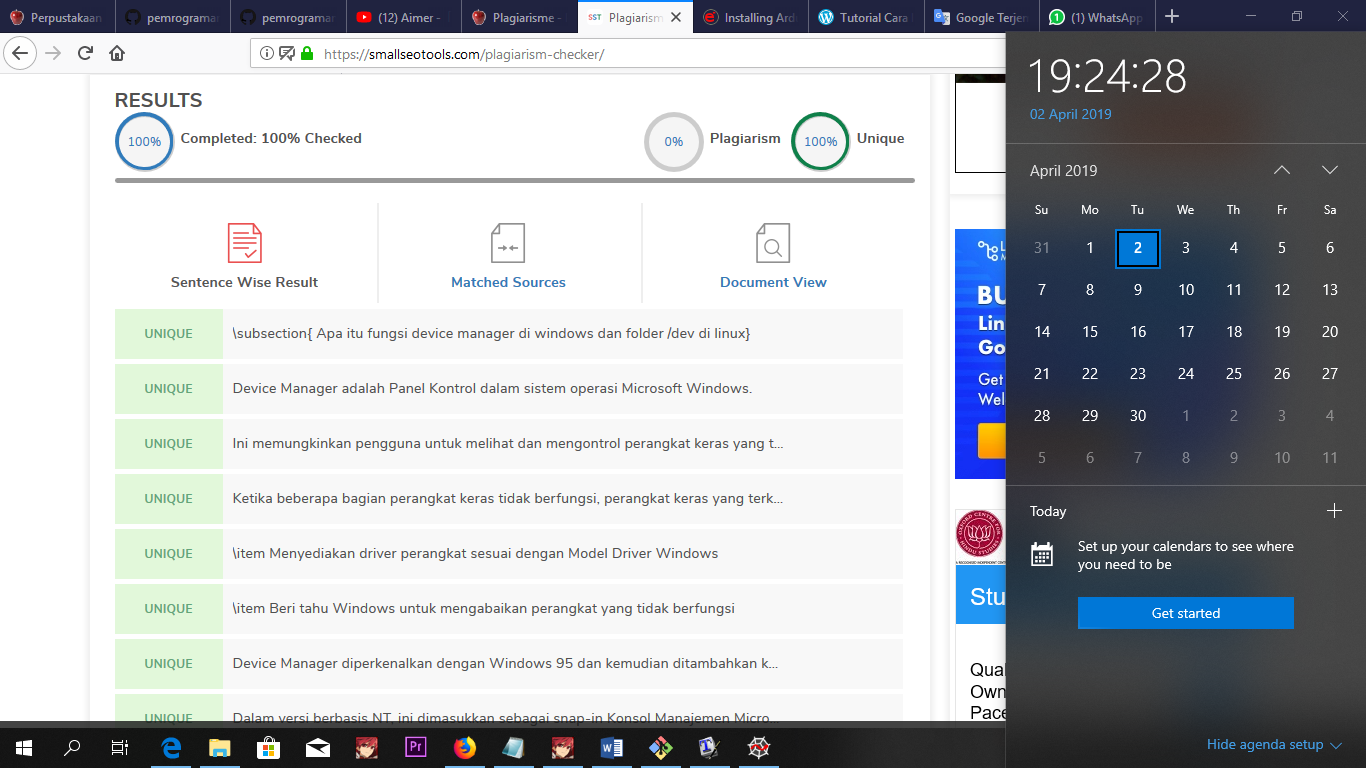
\includegraphics[scale=0.2]{figures/5/Teori/1174056/plagiat.png}
\caption{Plagiarisme}
\label{fig:plagiat}
\end{figure}

\section{Teddy Gideon Manik}
\subsection{Teori}
\subsubsection{Apa itu fungsi device manager di windows dan folder /dev di linux}
Fungsi device manager dan folder /dev itu berfungsi untuk mengetahui device apa saja yang telah terinstal di leptop anda serta mengetahui port yang digunakan oleh device tersebut.

\subsubsection{Jelaskan langkah-langkah instalasi driver dari arduino}
\begin{enumerate}
\item Cara Auto
\begin{itemize}
\item Pertama Hubungkan sistem minimum Arduino Uno ke komputer dengan kabel USB type B(kabel Printer)
\begin{figure}[H] 
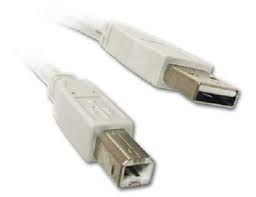
\includegraphics[width=5cm]{figures/5/Teori/1174038/1.jpg}
\centering
\caption{Membuat file csv}
\end{figure}

\item Lalu pada bagian kanan didesktop PC anda, akan muncul popup “Installing device driver software” seperti pada gambar dibawah ini.
\begin{figure}[H] 
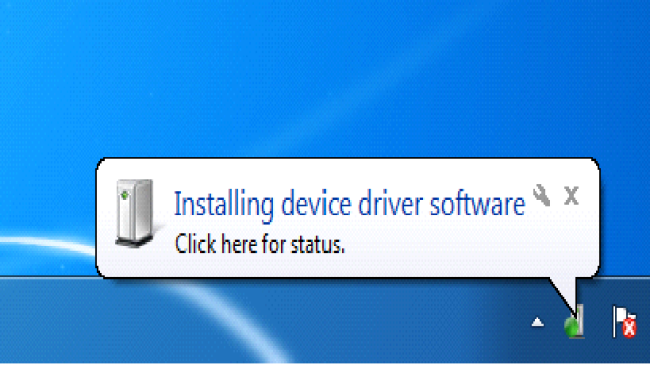
\includegraphics[width=5cm]{figures/5/Teori/1174038/2.png}
\centering
\caption{Membuat file csv}
\end{figure}

\item Tunggu hingga selesai.
\item Jika sudah selesai anda bisa mengecheck di device manager.
\begin{figure}[H] 
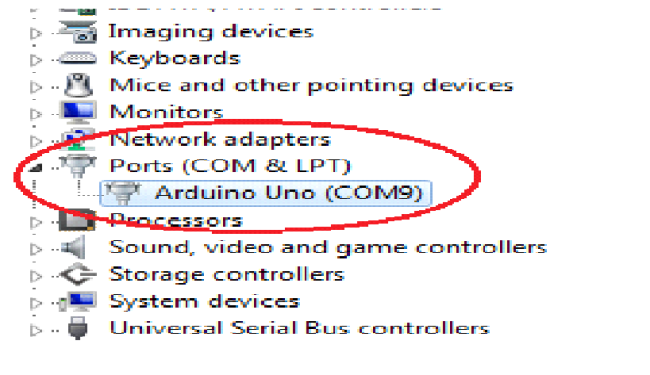
\includegraphics[width=5cm]{figures/5/Teori/1174038/11.png}
\centering
\caption{Membuat file csv}
\end{figure}
\end{itemize}

\item Cara Manual

\begin{itemize}
\item Penginstalan secara manual akan dilakukan jika penginstalan secara auto gagal dilakukan.
\item Buka Device Manager, caranya pada bagian Search Program and Files lalu ketikkan “device manager”, perhatikan gambar dibawah ini. Pada bagian Control Panel akan muncul Device Manager, klik untuk menjalankan.
\begin{figure}[H] 
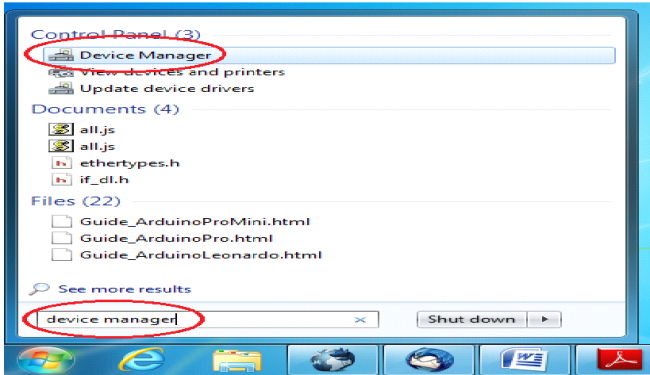
\includegraphics[width=5cm]{figures/5/Teori/1174038/4.png}
\centering
\caption{Membuat file csv}
\end{figure}

\item Cari Unknown device pada bagian Other device, biasanya terdapat tanda seru berwarna kuning, itu disebabkan karena penginstallan tidak berjalan dengan sempurna.
\begin{figure}[H] 
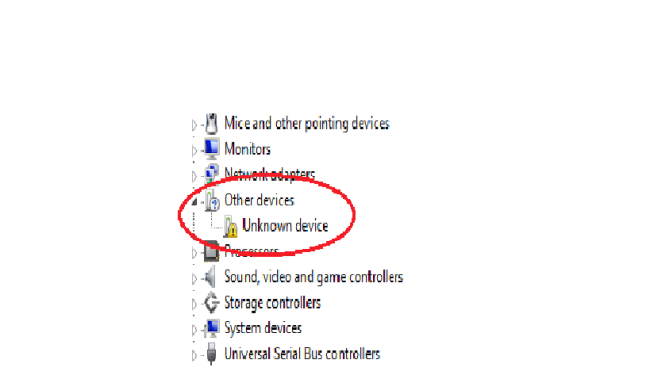
\includegraphics[width=5cm]{figures/5/Teori/1174038/5.png}
\centering
\caption{Membuat file csv}
\end{figure}

\item Klik kanan pada “Unknown device” kemudian pilih Update Driver Software.
\begin{figure}[H] 
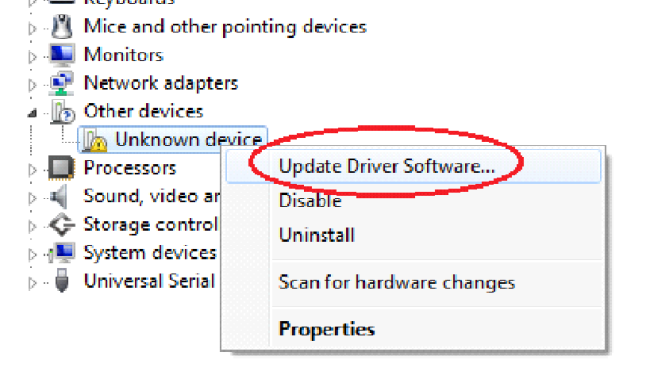
\includegraphics[width=5cm]{figures/5/Teori/1174038/6.png}
\centering
\caption{Membuat file csv}
\end{figure}

\item Pilih Browse my computer for driver software.
\begin{figure}[H] 
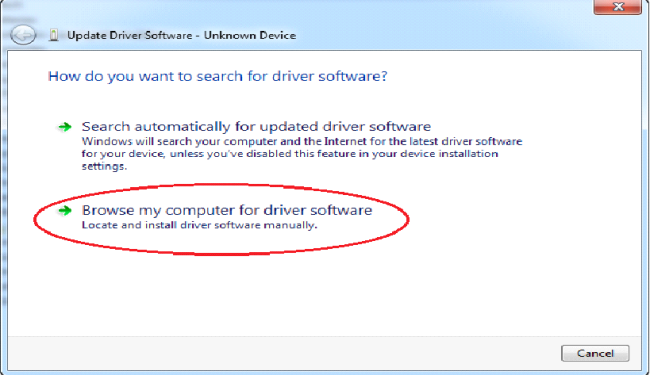
\includegraphics[width=5cm]{figures/5/Teori/1174038/7.png}
\centering
\caption{Membuat file csv}
\end{figure}

\item Arahkan lokasi folder ke folder ..arduino-1.0.5 drivers. Pastikan check-box lalu centang include subfolders. Klik Next untuk melanjutkan instalasi driver.
\begin{figure}[H] 
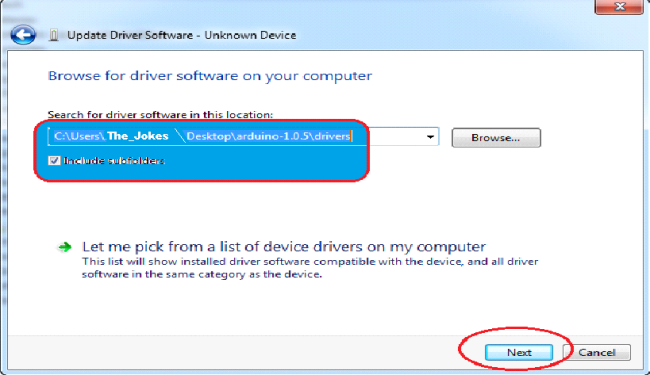
\includegraphics[width=5cm]{figures/5/Teori/1174038/8.png}
\centering
\caption{Membuat file csv}
\end{figure}

\item Kemudian lanjutkan dengan mengklik Install pada tampilan Windows Security.
\begin{figure}[H] 
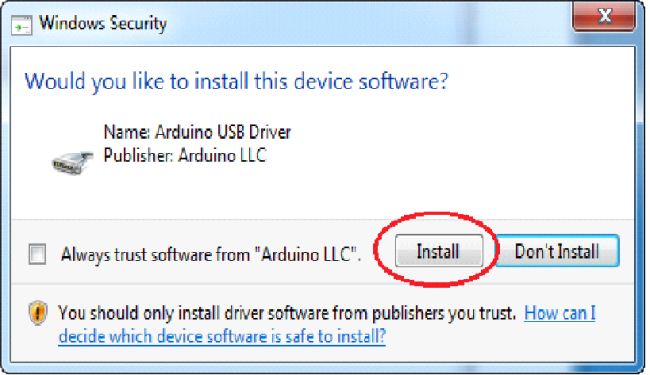
\includegraphics[width=5cm]{figures/5/Teori/1174038/9.png}
\centering
\caption{Membuat file csv}
\end{figure}

\item Jika instalasi driver berhasil maka akan muncul Windows has successfully updated your driver software.
\begin{figure}[H] 
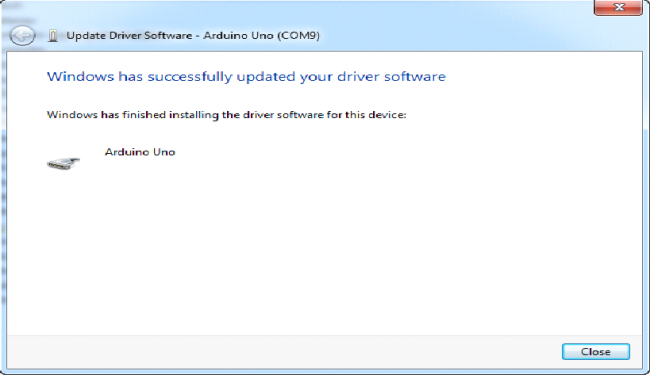
\includegraphics[width=5cm]{figures/5/Teori/1174038/10.png}
\centering
\caption{Membuat file csv}
\end{figure}

\item Perhatikan dan ingat nama COM Arduino Uno, karena nama COM ini yang akan digunakan untuk meng-upload program nantinya.
\begin{figure}[H] 
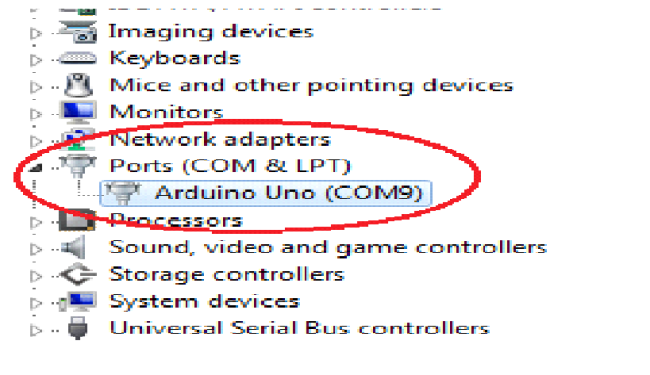
\includegraphics[width=5cm]{figures/5/Teori/1174038/11.png}
\centering
\caption{Membuat file csv}
\end{figure}
\end{itemize}
\end{enumerate}
\subsubsection{Jelaskan bagaimana cara membaca baudrate dan port dari komputer yang sudah terinstall driver}
Untuk baudrate itu bisa dicek melalui arduino IDE, kemudian untuk mengecheck port bisa dilakukan dengan device manager

\subsubsection{Jelaskan sejarah library pyserial}
Modul ini merangkum akses untuk port serial. Ini menyediakan backends untuk Python yang berjalan di Windows, Linux, BSD (mungkin sistem yang mendukung POSIX), Jython dan IronPython (.NET dan Mono). Modul bernama "serial" secara otomatis memilih backend yang sesuai. Antarmuka berbasis kelas yang sama pada semua platform yang didukung.
Akses ke pengaturan port melalui properti Python.
Dukungan untuk berbagai ukuran byte, bit stop, paritas dan kontrol aliran dengan RTS / CTS dan / atau Xon / Xoff.
Bekerja dengan atau tanpa menerima batas waktu.
File seperti API dengan "read" dan "write" ("readline" dll. Juga didukung).
File-file dalam paket ini adalah 100 persen Python murni.
Port diatur untuk transmisi biner. Tidak ada stripping byte NULL, terjemahan CR-LF dll. (Yang berkali-kali diaktifkan untuk POSIX.) Ini membuat modul ini bermanfaat secara universal.
Kompatibel dengan pustaka io (Python 2.6+)

\subsubsection{Jelaskan fungsi-fungsi apa saja yang dipakai dari library pyserial}


Serial – fungsi ini untuk membuka port serial
Write(data) – untuk menulis data lewat port serial
Readline() – untuk membaca string dari port serial
Read(size) – untuk membaca jumlah byte dari port serial
Close() – ini untuk menutup port serial 

\subsubsection{Jelaskan kenapa butuh perulangan dan tidak butuh perulangan dalam membaca serial}


Perualangan dalam bahasa pemrograman berfungsi menyuruh komputer melakukan sesuatu secara berulang-ulang. Terdapat dua jenis perualangan dalam bahasa pemrograman python, yaitu perulangan dengan for dan while.
Perulangan for disebut counted loop (perulangan yang terhitung), sementara perulangan while disebut uncounted loop (perulangan yang tak terhitung). Perbedaannya adalah perulangan for biasanya digunakan untuk mengulangi kode yang sudah diketahui banyak perulangannya. Sementara while untuk perulangan yang memiliki syarat dan tidak tentu berapa banyak perulangannya.
Perulangan diperlukan agar dapat membaca data secara berulang kali sehingga data yang muncul lebih dari satu. Sedangkan apabila tidak memakai perulangan maka data akan terbaca satu kali saja.

\subsubsection{Jelaskan bagaimana cara membuat fungsi yang mengunakan pyserial}

\hfill \break
Fungsi yang berada pada Python, dibuat dengan nama kata kunci def kemudian diikuti dengan nama fungsinya pada pyhton.
Seperti halnya dengan blok kode yang lain, kita juga harus memberikan identasi untuk menuliskan isi fungsi.

\subsubsection{Scan Plagiarisme}
\begin{figure}[H] 
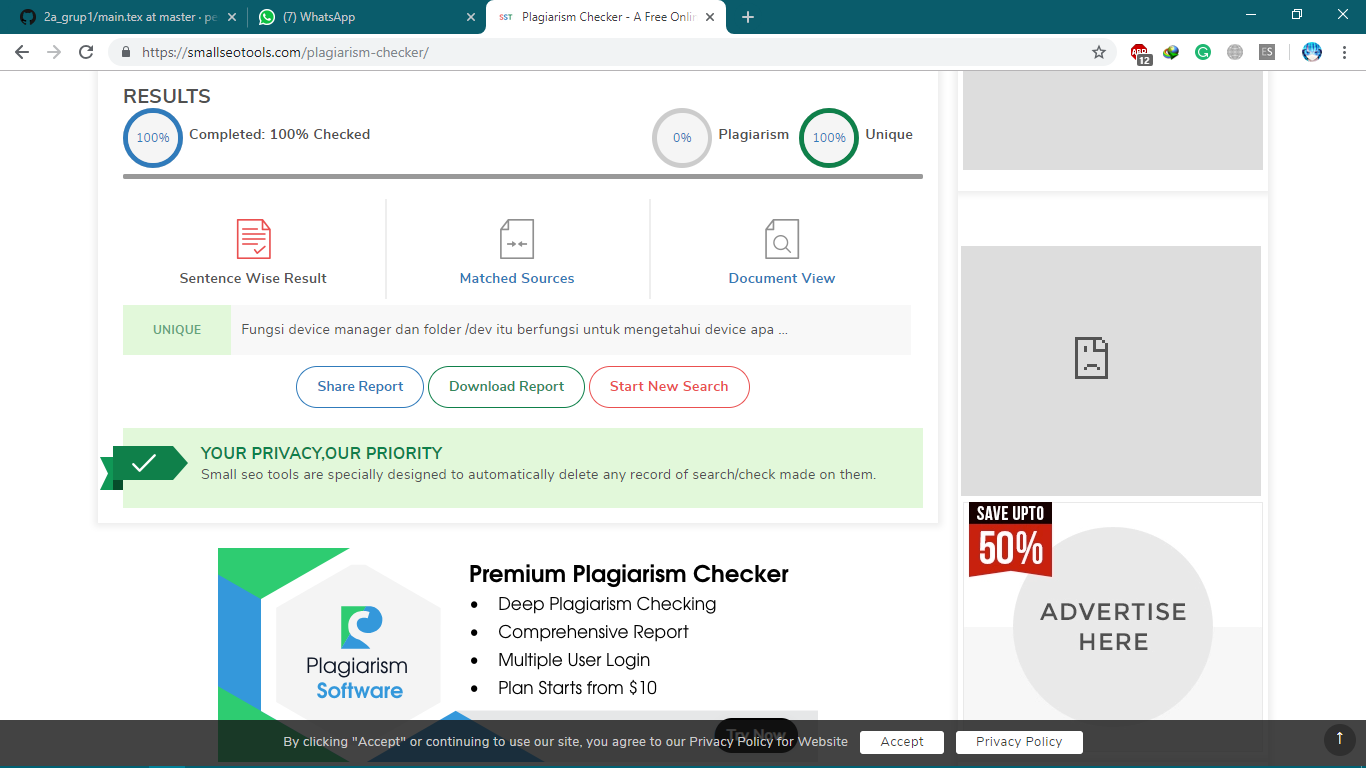
\includegraphics[width=5cm]{figures/5/Teori/1174038/nopla.png}
\centering
\caption{Membuat file csv}
\end{figure}

\subsection{Praktek}
\subsubsection{Kerjakan soal berikut ini, ....}
\subsubsection{Penanganan Error}
%PRAKTEK
\chapter{Praktek PySerial}
\section{LIYANA MAJDAH RAHMA 1174039}
{\Large \textbf{Ketrampilan Pemrograman}}
\subsection{Soal No. 1}
Buatlah  fungsi  (file  terpisah/library  dengan  nama  NPMrealtime.py)  untuk mendapatkan data langsung dari arduino!
\lstinputlisting[caption = Fungsi untuk mendapatkan data dari Arduino., firstline=1, lastline=7]{src/5/1174039/Praktek/1174039realtime.py}

\begin{figure}[H]
	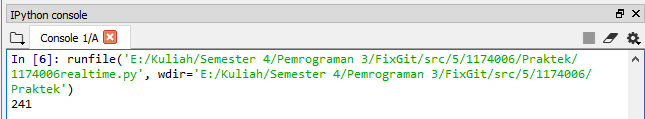
\includegraphics[width=12cm]{figures/5/1174039/Praktek/1.png}
	\centering
	\caption{Hasil dari pembacaan fungsi untuk mendapatkan data dari Arduino.}
\end{figure}

\subsection{Soal No. 2}
Buatlah fungsi (file terpisah/library dengan nama NPMsave.py) untuk mendapatkan data langsung dari arduino dengan looping!
\lstinputlisting[caption = Fungsi untuk mendapatkan data langsung dari Arduino dengan looping., firstline=1, lastline=8]{src/5/1174039/Praktek/1174039save.py}

\begin{figure}[H]
	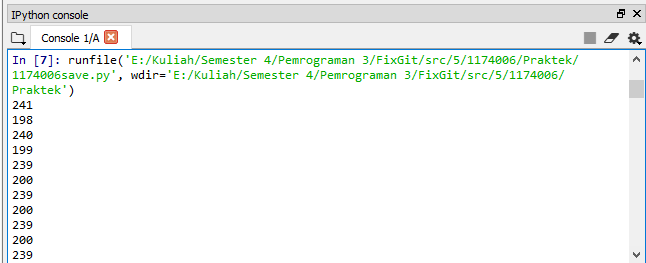
\includegraphics[width=12cm]{figures/5/1174039/Praktek/2.png}
	\centering
	\caption{Hasil dari pembacaan fungsi untuk mendapatkan data dari Arduino dengan looping.}
\end{figure}

\subsection{Soal No. 3}
Buatlah  fungsi  (file  terpisah/library  dengan  nama  NPMrealtime.py) untuk mendapatkan data dari arduino dan langsung ditulis kedalam file csv!
\lstinputlisting[caption = Fungsi untuk mendapatkan data dari Arduino dan langsung ditulis kedalam file CSV., firstline=9, lastline=23]{src/5/1174039/Praktek/1174039realtime.py}

\begin{figure}[H]
	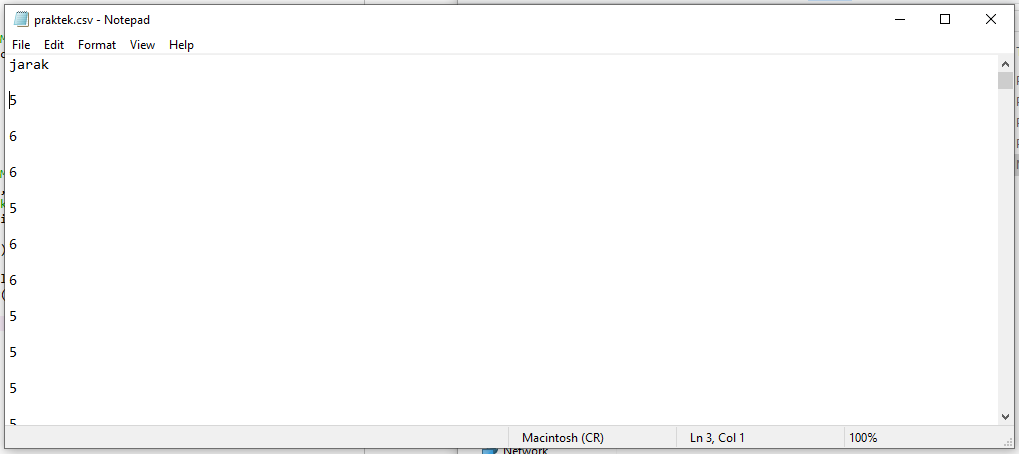
\includegraphics[width=12cm]{figures/5/1174039/Praktek/3.png}
	\centering
	\caption{Hasil dari pembacaan fungsi untuk mendapatkan data dari Arduino dan langsung ditulis kedalam file CSV.}
\end{figure}

\subsection{Soal No. 4}
Buatlah fungsi (file terpisah/library dengan nama NPMcsv.py) untuk membaca file csv hasil arduino dan mengembalikan ke fungsi!
\lstinputlisting[caption = Fungsi untuk membaca file CSV hasil Arduino dan mengembalikan fungsi., firstline=1, lastline=9]{src/5/1174039/Praktek/1174039csv.py}

\begin{figure}[H]
	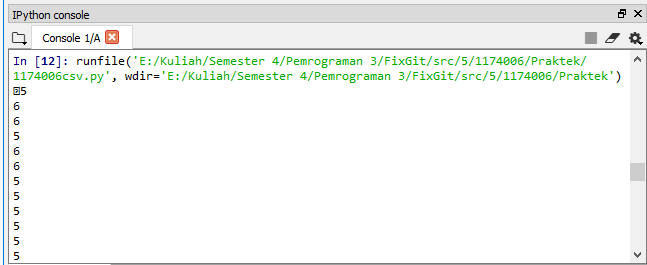
\includegraphics[width=12cm]{figures/5/1174039/Praktek/4.png}
	\centering
	\caption{Hasil dari pembacaan fungsi untuk membaca file csv hasil arduino dan mengembalikan fungsi.}
\end{figure}

\subsection{Kode Program Praktek}
\begin{figure}[H]
	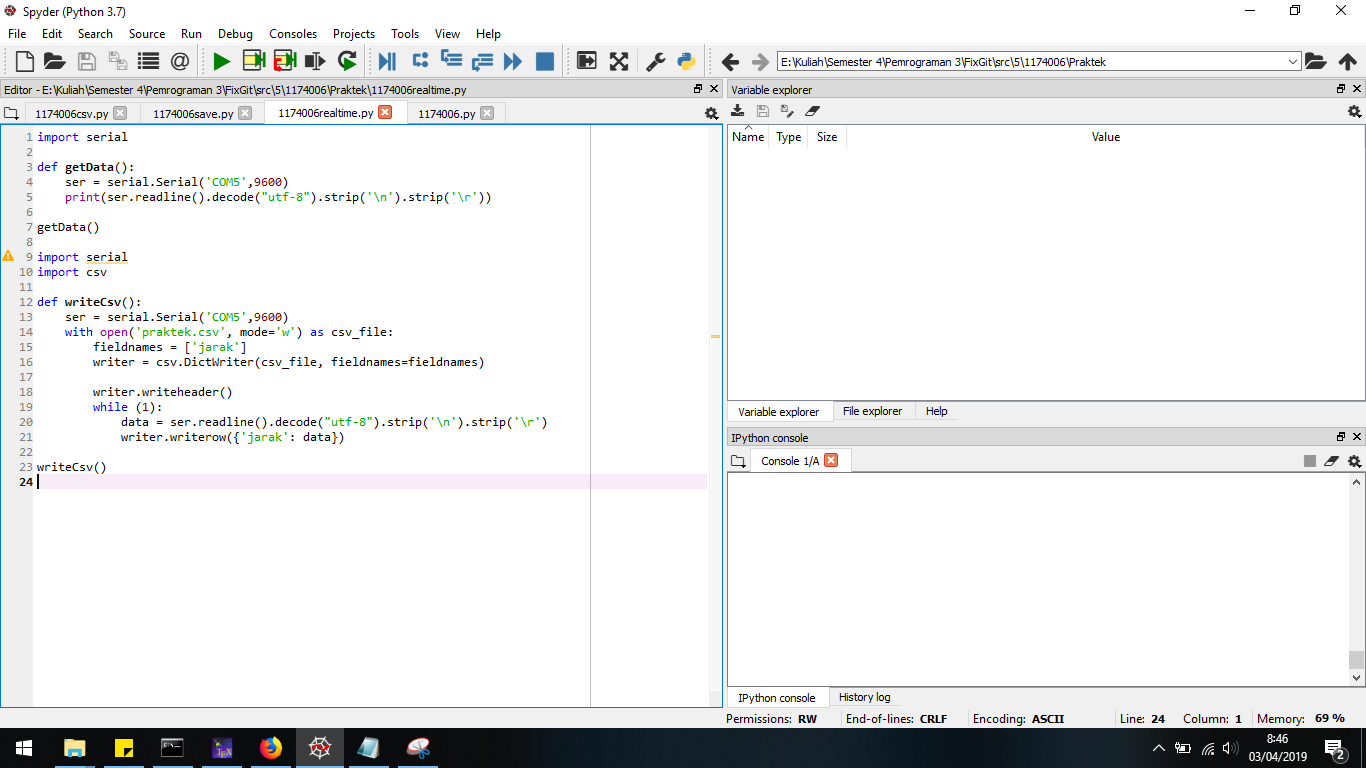
\includegraphics[width=9cm]{figures/5/1174039/Praktek/realtime.png}
	\centering
\end{figure}

\begin{figure}[H]
	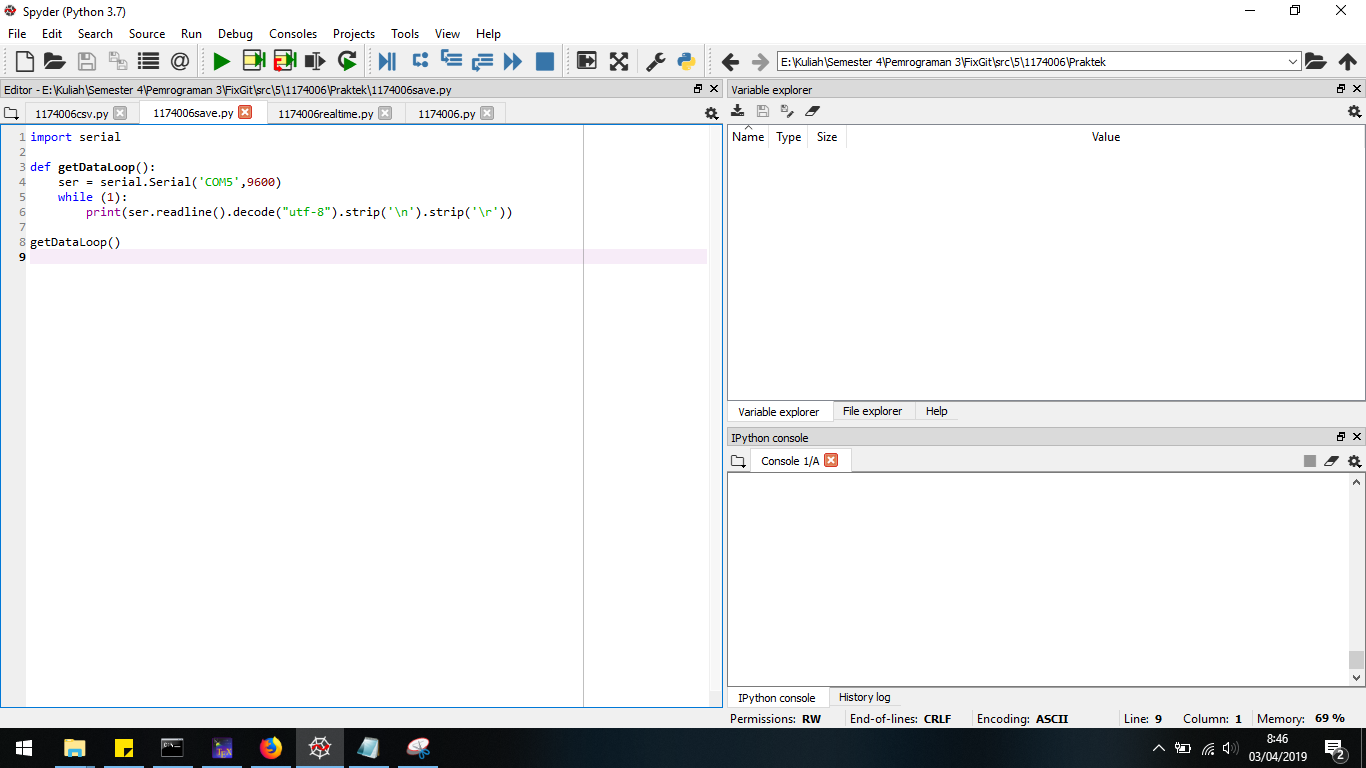
\includegraphics[width=9cm]{figures/5/1174039/Praktek/save.png}
	\centering
\end{figure}

\begin{figure}[H]
	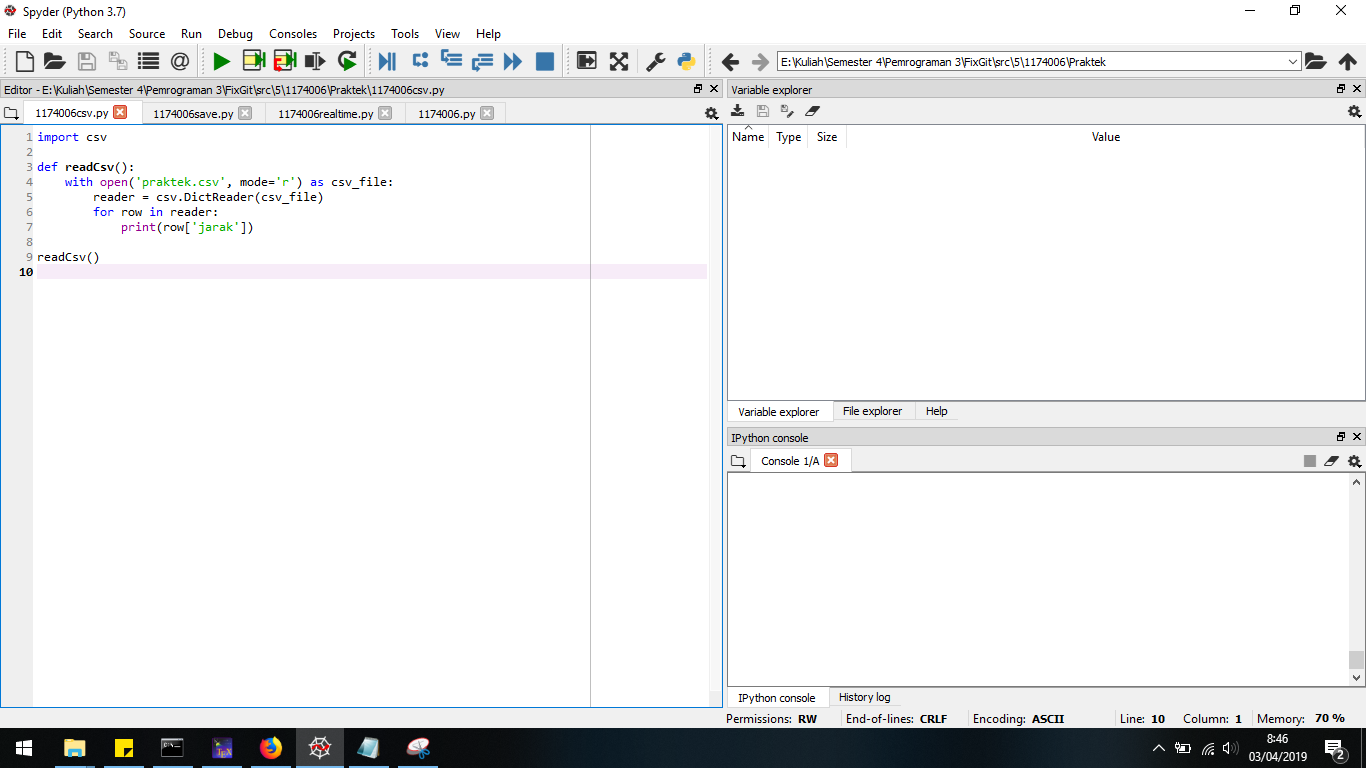
\includegraphics[width=9cm]{figures/5/1174039/Praktek/csv.png}
	\centering
\end{figure}

\subsection{Cek Plagiat Praktek}
\begin{figure}[H]
	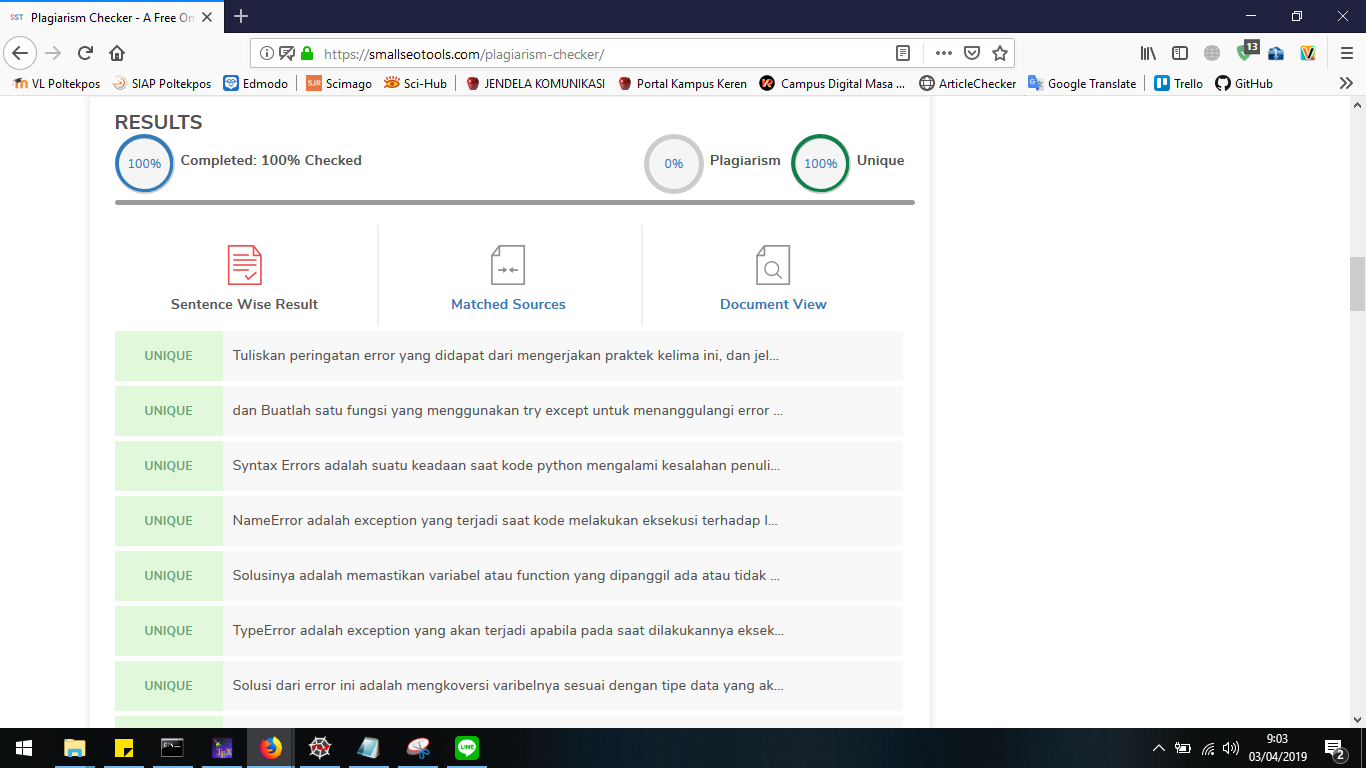
\includegraphics[width=9cm]{figures/5/1174039/Praktek/plagiat.png}
	\centering
\end{figure}

\hfill \break
{\Large \textbf{Ketrampilan Penanganan Error}}

\subsection{Soal No. 1}
Tuliskan  peringatan  error  yang  didapat  dari  mengerjakan  praktek  kelima  ini, dan  jelaskan  cara  penanganan  error  tersebut.   dan  Buatlah  satu  fungsi  yang menggunakan try except untuk menanggulangi error tersebut.

\hfill \break
Peringatan error di praktek kelima ini, yaitu:
\begin{itemize}
	\item Syntax Errors
	Syntax Errors adalah suatu keadaan saat kode python mengalami kesalahan penulisan. Solusinya adalah memperbaiki penulisan kode yang salah.
	
	\item Name Error
	NameError adalah exception yang terjadi saat kode melakukan eksekusi terhadap local name atau global name yang tidak terdefinisi. Solusinya adalah memastikan variabel atau function yang dipanggil ada atau tidak salah ketik.
	
	\item Type Error
	TypeError adalah exception yang akan terjadi apabila pada saat dilakukannya eksekusi terhadap suatu operasi atau fungsi dengan type object yang tidak sesuai. Solusi dari error ini adalah mengkoversi varibelnya sesuai dengan tipe data yang akan digunakan.
\end{itemize}

\hfill \break
Fungsi yang menggunakan try except untuk menanggulangi error.

\lstinputlisting[caption = Fungsi untuk menanggulangi error menggunakan Try Except., firstline=1, lastline=16]{src/5/1174039/Praktek/1174039.py}

\begin{figure}[H]
	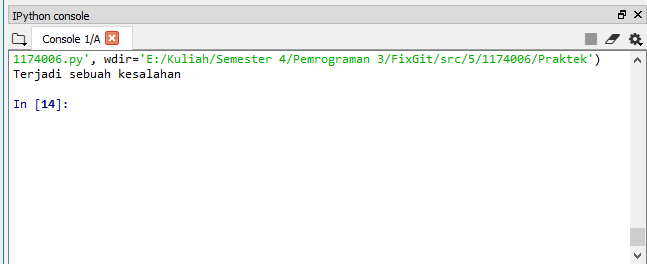
\includegraphics[width=12cm]{figures/5/1174039/Praktek/5.png}
	\centering
	\caption{Hasil pembacaan fungsi untuk menanggulangi error menggunakan Try Except.}
\end{figure}

\subsection{Kode Program Penanganan Error}
\begin{figure}[H]
	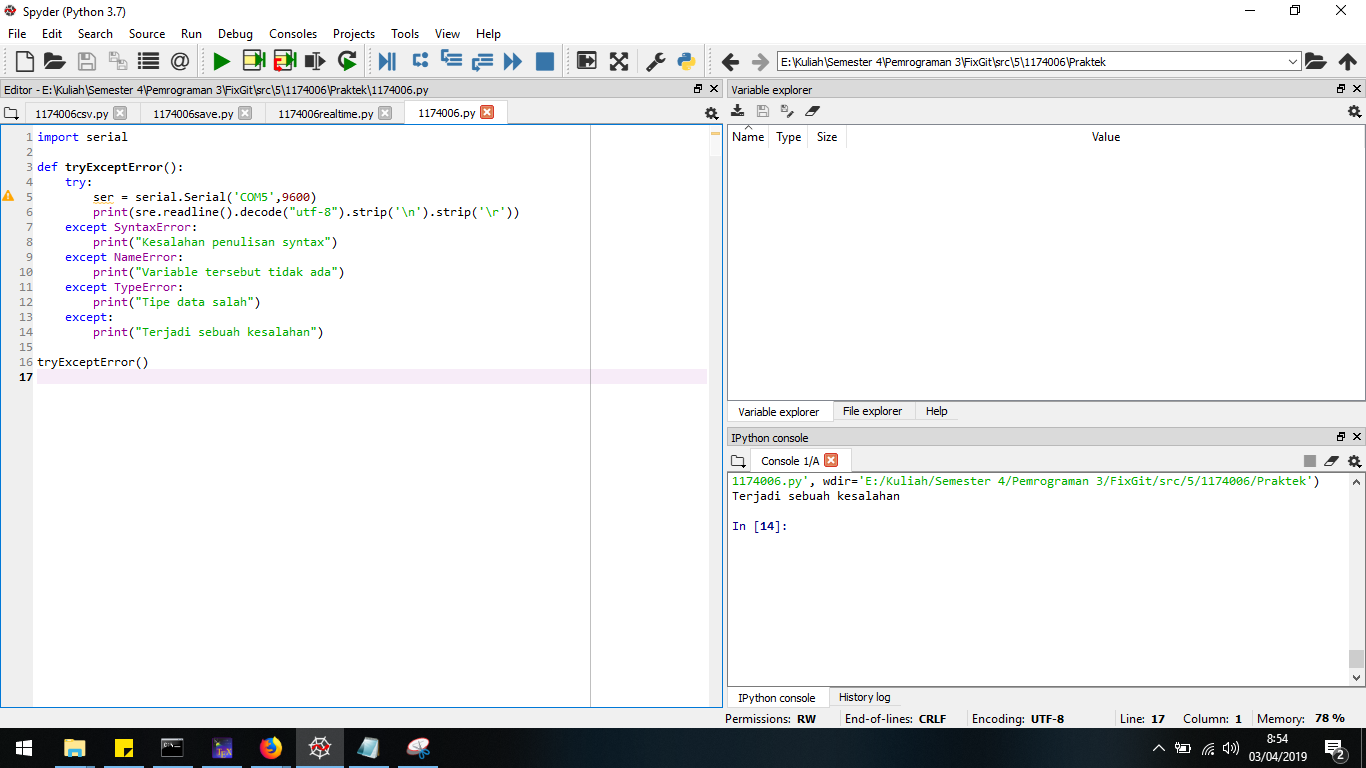
\includegraphics[width=12cm]{figures/5/1174039/Praktek/error.png}
	\centering
\end{figure}

\subsection{Cek Plagiat Penanganan Error}
\begin{figure}[H]
	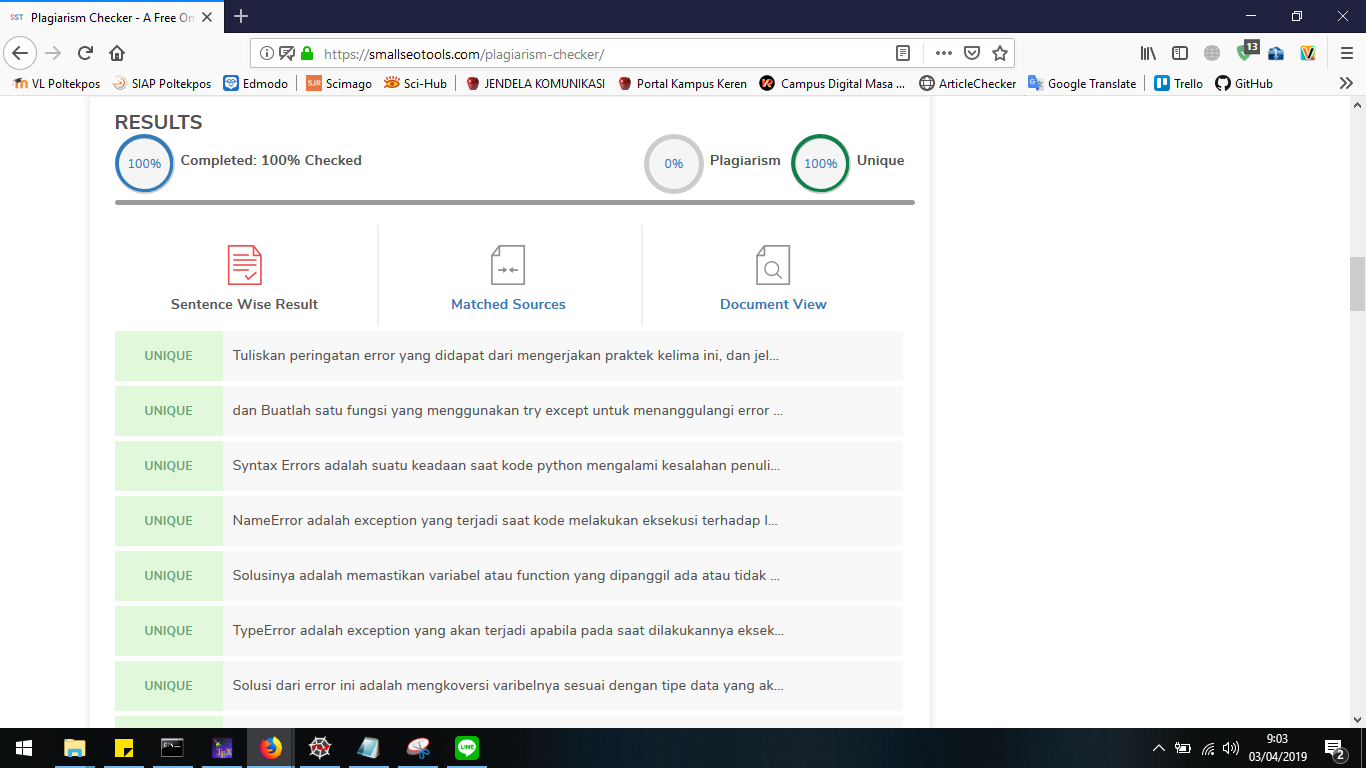
\includegraphics[width=12cm]{figures/5/1174039/Praktek/plagiat.png}
	\centering
\end{figure}

\bibliographystyle{IEEEtran}
%\def\bibfont{\normalsize}
\bibliography{references}


%%%%%%%%%%%%%%%
%%  The default LaTeX Index
%%  Don't need to add any commands before \begin{document}
\printindex

%%%% Making an index
%%
%% 1. Make index entries, don't leave any spaces so that they
%% will be sorted correctly.
%%
%% \index{term}
%% \index{term!subterm}
%% \index{term!subterm!subsubterm}
%%
%% 2. Run LaTeX several times to produce <filename>.idx
%%
%% 3. On command line, type  makeindx <filename> which
%% will produce <filename>.ind
%%
%% 4. Type \printindex to make the index appear in your book.
%%
%% 5. If you would like to edit <filename>.ind
%% you may do so. See docs.pdf for more information.
%%
%%%%%%%%%%%%%%%%%%%%%%%%%%%%%%

%%%%%%%%%%%%%% Making Multiple Indices %%%%%%%%%%%%%%%%
%% 1.
%% \usepackage{multind}
%% \makeindex{book}
%% \makeindex{authors}
%% \begin{document}
%%
%% 2.
%% % add index terms to your book, ie,
%% \index{book}{A term to go to the topic index}
%% \index{authors}{Put this author in the author index}
%%
%% \index{book}{Cows}
%% \index{book}{Cows!Jersey}
%% \index{book}{Cows!Jersey!Brown}
%%
%% \index{author}{Douglas Adams}
%% \index{author}{Boethius}
%% \index{author}{Mark Twain}
%%
%% 3. On command line type
%% makeindex topic
%% makeindex authors
%%
%% 4.
%% this is a Wiley command to make the indices print:
%% \multiprintindex{book}{Topic index}
%% \multiprintindex{authors}{Author index}

\end{document}

